\documentclass[a4paper,14pt]{article}
\usepackage{amsmath}
\usepackage[utf8]{inputenc} % 
\usepackage{graphicx}
\graphicspath{{img/}}
\DeclareGraphicsExtensions{.png,.jpg}
\usepackage{multicol}

\usepackage[russian]{babel} % правила переноса
\usepackage[left=2cm,right=2cm,
top=2cm,bottom=2cm,bindingoffset=0cm]{geometry} % для изменения размеров полей документа
\usepackage{commath}
\usepackage{listings}
\usepackage[framed,numbered,autolinebreaks,useliterate]{mcode}

\begin{document}

%%%%%%%%%%%%%%%%%%%%%% Титульный лист %%%%%%%%%%%%%%%%%%%%%%

\begin{titlepage}
	\newpage
	
	\begin{center}
		Санкт-Петербургский государственный политехнический 
		университет Петра Великого \\
		\vspace{1cm}
		Кафедра компьютерных систем и программных технологий\\*
%		\hrulefill
	\end{center}
	
	\vspace{8em}
	
	\begin{center}
		 Отчёт по лабораторной работе № 3
	\end{center}
	
	\vspace{2.5em}

	\vspace{6em}
	\flushleft{Выполнила студентка гр.33501/3:Ивашкевич О.А.}

	\flushleft{Преподаватель: Богач Н.В.}
	\vspace{\fill}
	
	\begin{center}
		Санкт-Петербург
		
		 2017
	\end{center}
	
\end{titlepage}


\newpage

\tableofcontents

\newpage

\section{Лабораторная работа №3. Линейная фильтрация}
%\setcounter {section}{0}
%\setcounter {equation}{0}
%\setcounter {figure}{0}
\subsection{Цель работы}
\hspace{0,5cm}  Изучить воздействие ФНЧ на тестовый сигнал с шумом.
\subsection{Постановка задачи}
\hspace{0,5cm}	 Сгенерировать гармонический сигнал с шумом
и синтезировать ФНЧ. Получить сигнал во временной и частотной
областях до и после фильтрации. Сделать выводы о воздействии
ФНЧ на спектр сигнала.

\subsection{Теоретическое обоснование}

\hspace{0,5cm}\textbf{Дискретный фильтр} - это произвольная система обработки дискретного сигнала, обладающая свойствами линейности и стационарности. \\

\textit{Линейность} значит, что выходная реакция на сумму сигналов равна сумме реакций на данные сигналы, поданные на вход по отдельности, а \textit{стационарность} - собственно задержка входного сигнала приводит только к такой же задержке выходного сигнала, не меняя его формы.
Чтобы обеспечить линейность и стационарность, производимые фильтром
математические операции должны ограничиваться сложением и умножением на
константы.\\

В общем случае дискретный фильтр суммирует (с весовыми коэффициентами) некое количество входных отсчетов (включая заключительный) и некоторое
число предыдущих входных отсчетов:

\begin{equation}
		y(k) = b_0 x(k) + b_1 x(k-1)+...+b_m x(k-m)-a_1 y(k-1)-a_2 y(k-2)-...-a_n y(k-n),
\end{equation}
где $a_1$ и $b_1$ - вещественные коэффициенты.\\

Формула (\theequation) величается \textit{методом дискретной фильтрации}. Если
по-иному сгруппировать слагаемые, чтобы с одной стороны от знака равенства были только входные отсчеты, а с иной — исключительно выходные, получим форму записи, именуемую \textit{разностным уравнением}:

\begin{equation}
		y(k) + a_1 y(k-1)+a_2 y(k-2)+...+a_n y(k-n) = b_0 x(k) + b_1 x(k-1)+...+b_m x(k-m).
\end{equation}

\subsubsection{Импульсная характеристика}

Дискретные системы, как и аналоговые, могут описываться разными
методами. Благодаря сходству параметров z-преобразования со свойствами преобразований Лапласа и Фурье приемы описания аналоговых и дискретных систем как правило смахивают друг на друга. \\

В случае линейных систем с неизменными параметрами для анализа
прохождения любого сигнала достаточно знать итог прохождения элементарного импульса повторяющий вид дельта-функции. Для дискретных систем помимо прочего можно ввести в рассмотрение \textit{единичную импульсную функцию} $x_0(k)$.  Выходная реакция на единичный импульс $x_0(k)$ называется \textit{импульсной
характеристикой дискретной системы} и обозначается $h(k)$.\\

Случайный сигнал $\{x(k)\}$ можно представить в виде линейной комбинации единичных отсчетов:

\[
	x(k) = \sum_{m=-\infty}^\infty x(m) x_0 (k-m) \quad
\]

Для того, чтобы выходной сигнал представлял собой линейную комбинацию импульсных характеристик, в нашей физически реализуемой системе $h(k) = 0$ при $k < 0$ необходимо  верхний предел суммирования можно заменить на $k$. 
Тем самым, система, при вычислении очередного отсчета оперирует только предыдущими значениями входного сигнала:


\begin{equation}
	x(k) = \sum_{m=-\infty}^k x(m) h (k-m) 
\end{equation}
Выражение (\theequation) является \textit{линейной дискретной сверткой}.\\

Рассматривая уравнение дискретной фильтрации, видно, что она представляет собой дискретную свертку, а значит,, согласно свойствам z-преобразования, результатом будет являться произведение z-преобразований:
\begin{equation}
	Y(z) = H(z)X(z),
\end{equation}

где $H(z)$ - \textbf{функция передачи} или \textbf{системная функция} дискретной системы:
\begin{equation}
	H(z) = \frac{Y(z)}{X(z)} = \sum_{k=0}^\infty h(k) z^{-k}
\end{equation}

\subsubsection{Нерекурсивные фильтры}
Нерекурсивные фильтры - фильтры, суммирующие некоторое число входных отсчетов, умножая их при этом на постоянные весовые коэффициенты, не учитывающие предыдущие значения выходного сигнала.\\

В КИХ фильтрах, при вычислении очередного выходного отсчета $y(k)$ используется информация двух типов: 
1)некоторое количество отсчетов входного сигнала 
2)некоторое количество предыдущих отсчетов выходного сигнала. 
Причем, Хотя бы один отсчет входного сигнала должен участвовать в вычислениях; 
иначе выходной сигнал не будет зависеть от входного. В противоположность этому, предыдущие отсчеты выходного сигнала могут и не использоваться. Уравнение фильтрации в этом случае приобретает следующий вид:

\begin{equation}
	y(k) = \sum_{i=0}^m b_i x(k-i) \quad
\end{equation}
Количество используемых предыдущих отсчетов $m$ называется \textit{порядком фильтра}. Ниже приведена структурная схема, реализующая алгоритм (\theequation):

\begin{figure}[bh]
\noindent\centering{
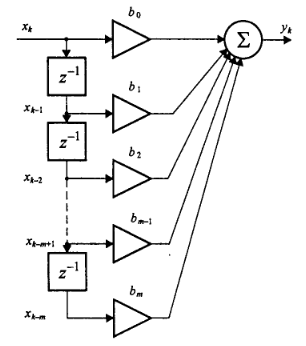
\includegraphics[width=50mm]{iir}}
\caption{Нерекурсивный фильтр}
\label{figCurves}
\end{figure}

Для определения \textit{импульсной характеристики нерекурсивного} фильтра необходимо подставить в уравнение (\theequation) единичный импульс $x_0(k)$ в качестве входного сигнала. Отсчет$x_0(k-i)$ равен нулю для всех k, кроме $k=i$, когда этот отсчет равен единице. В результате получаем:

\begin{equation}
	h(k) = \sum_{i=0}^m b_i x_0(k-i)=b_k. \quad
\end{equation}
 Коэффициенты  $b_i$, являются отсчетами импульсной характеристики фильтра.Так как в реальном устройстве линия задержки содержит конечное число элементов, отсюда импульсная характеристика нерекурсивного фильтра также является конечной по длительности. Это обусловило еще одно название таких фильтров —
фильтры с \textit{конечной импульсной характеристикой} (КИХ-фильтры; английский термин — finite impulse response, FIR).

\subsubsection{Рекурсивные фильтры}
Главная отличительная черта рекурсивных фильтров - использование при вычислениях предыдущий отсчет выходного сигнала. \\
Для реализации такого фильтра в схему, приведенную на рис. (\ref{figCurves}), необходимо добавить вторую линию задержки — для хранения выходных отсчетов $y(k - i)$. Получившаяся при этом структура представлена ниже:

\begin{figure}[bh]
\noindent\centering{
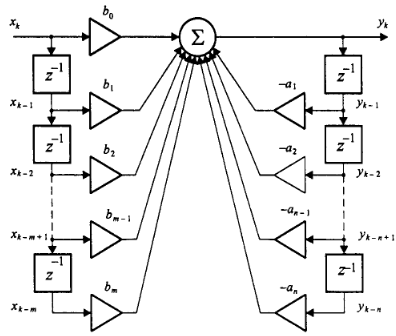
\includegraphics[width=70mm]{fir}}
\caption{Рекурсивный фильтр}
\label{figCurves}
\end{figure}

Так как в схеме есть обратные связи, тогда возможно получить бесконечную импульсную характеристику, благодаря этому свойству, рекурсивные фильтры называют также фильтрами с
\textit{бесконечной импульсной характеристикой} (БИХ-фильтрами; английский термин — infinite impulse response, IIR). По этой же причине рекурсивные фильтры могут быть неустойчивыми.
\newpage
\subsection{Ход работы}

Генерация гармонического сигнала и добавление к нему белого шума:
\begin{lstlisting}
Fs =   2000;
F = 1;
t = 0 : 1/Fs: 5; 
A = 2; 
s = A * sin(2*pi*F*t);	
y = awgn(s,20); 		
\end{lstlisting}

\hspace{0,5cm}Ниже показан вид полученного сигнала во временной и частотной областях:

\begin{figure}[h]
\begin{multicols}{1}
\hfill
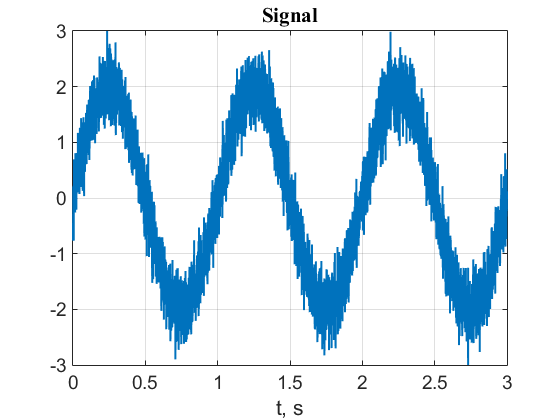
\includegraphics[width=90mm]{noisy}
\hfill
\caption{Зашумленный сигнал}
\label{figBottom}
\hfill
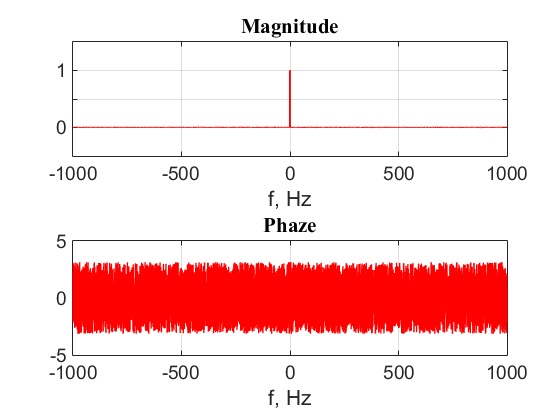
\includegraphics[width=100mm]{noisy_spec}
\hfill
\caption{Спектры замушленного сигнала}
\label{figDown}
\end{multicols}
\end{figure}

\newpage
\hspace{0,5cm}Синтезируем ФНЧ Кайзера посредством программы FDATool:
\begin{figure}[bh]
\noindent\centering{
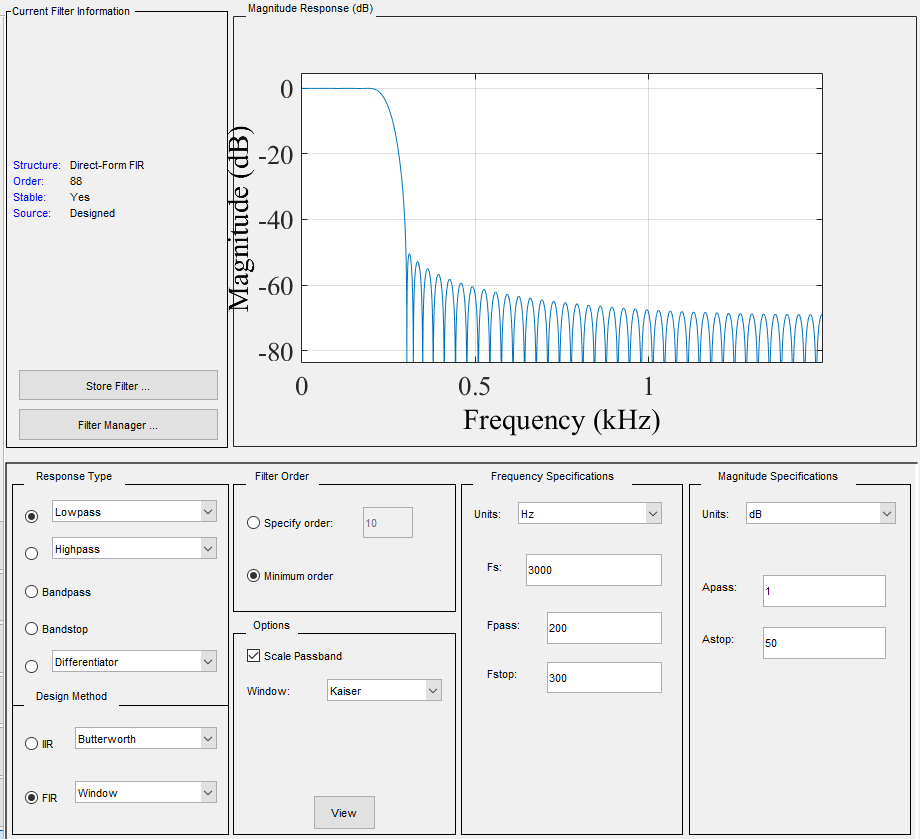
\includegraphics[width=150mm]{fdatool}}
\caption{Окно программы FDATool}
\label{figCurves}
\end{figure}

\hspace{0,5cm}В результате был создан фильтр $88$ порядка и сгенерирован код в $Matlab$ для нахождения коэффициентов уравнения фильтрации:

\begin{lstlisting}
Fs = 3000;  % Sampling Frequency
Fpass = 200;                % Passband Frequency
Fstop = 300;              % Stopband Frequency
Dpass = 0.057501127785;   % Passband Ripple
Dstop = 0.0031622776602;  % Stopband Attenuation
flag  = 'scale';          % Sampling Flag

% Calculate the order from the parameters using KAISERORD.
[N,Wn,BETA,TYPE] = kaiserord([Fpass Fstop]/(Fs/2), [1 0], [Dstop Dpass]);

% Calculate the coefficients using the FIR1 function.
b  = fir1(N, Wn, TYPE, kaiser(N+1, BETA), flag);
Hd = dfilt.dffir(b);
\end{lstlisting}
%\newpage
Осуществим свёртку зашумленного сигнала с полученной импульсной функцией $h(k) = b_k$, а также с помощью функции $filter$:

\begin{lstlisting}
yy=filter(b,1,y)
figure; plot(yy,'linewidth', 1.5);
grid on;
spectrum(Fs,t,yy);
yy=conv(y,b)
figure; plot(yy,'linewidth', 1.5);
spectrum(Fs,t,yy);
grid on;
\end{lstlisting}
\hspace{0,5cm} В обоих случаях получен одинаковый результат:

\begin{figure}[h]
\begin{multicols}{1}
\hfill
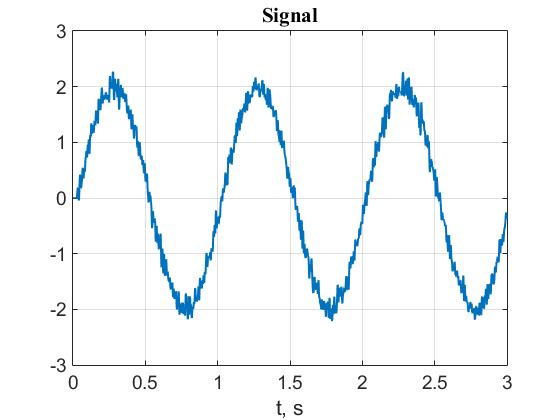
\includegraphics[width=90mm]{filtered}
\hfill
\caption{Отфильтрованный сигнал}
\label{figBottom}
\hfill
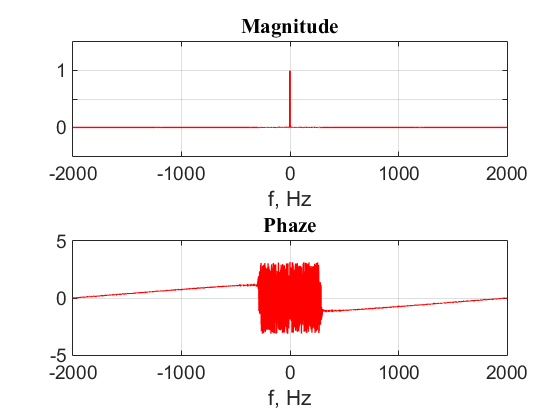
\includegraphics[width=100mm]{filtered_spec}
\hfill
\caption{Спектры отфильтрованного сигнала}
\label{figDown}
\end{multicols}
\end{figure}

Как видно, в сигнале присутствуют шумы, значит фильтр не справляется со своей задачей. Проведем улучшение, увеличив частоту дискретизации до 4000, также уменьшим полосу пропускания.
\newpage
\begin{figure}[bh]
	\noindent\centering{
		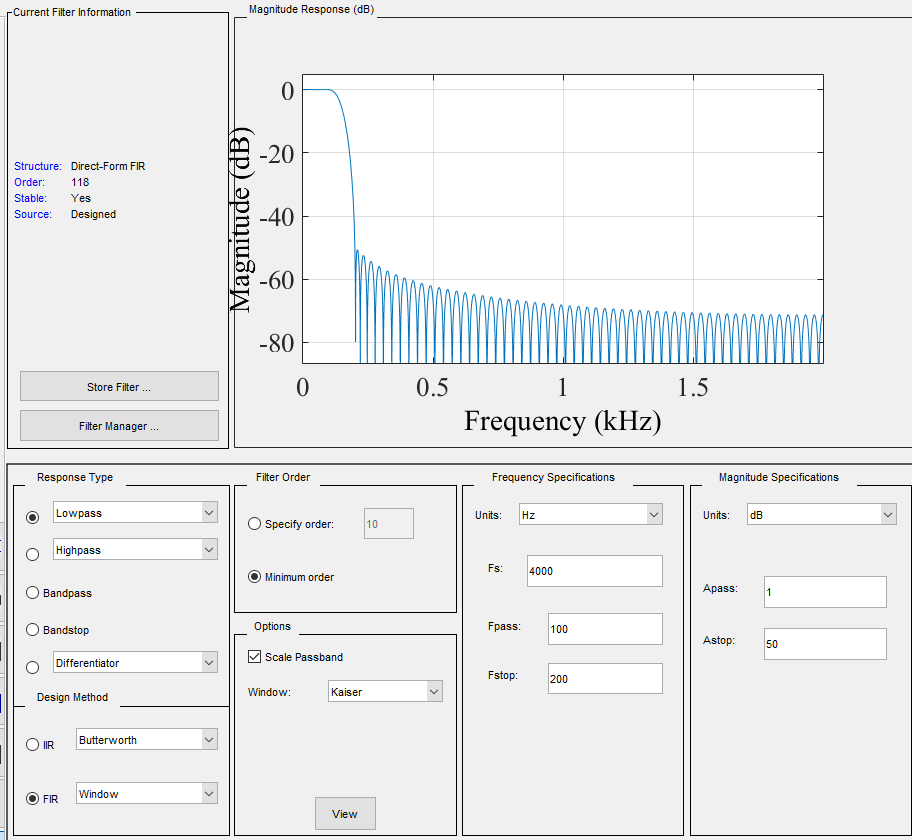
\includegraphics[width=150mm]{fdatool2}}
	\caption{Окно программы FDATool}
	\label{figCurves}
\end{figure}

\hspace{0,5cm}В результате был синтезирован фильтр $118$ порядка. Рассмотрим отфильтрованный сигнал.

\newpage
\begin{figure}[h]
	\begin{multicols}{1}
		\hfill
		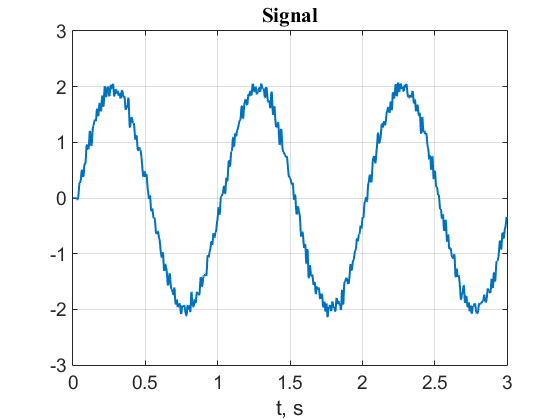
\includegraphics[width=90mm]{filtered2}
		\hfill
		\caption{Отфильтрованный сигнал}
		\label{figBottom}
		\hfill
		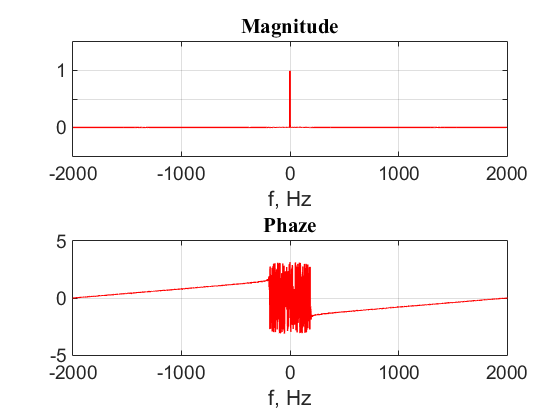
\includegraphics[width=100mm]{filtered_spec2}
		\hfill
		\caption{Спектры отфильтрованного сигнала}
		\label{figDown}
	\end{multicols}
\end{figure}

\hspace{0,5cm} Как видно, шум все еще присутствует в сигнале, однако его воздействие меньше, чем при фильтре $88$ порядка. Продолжим уменьшение частоты пропускания.

\newpage
\begin{figure}[bh]
	\noindent\centering{
		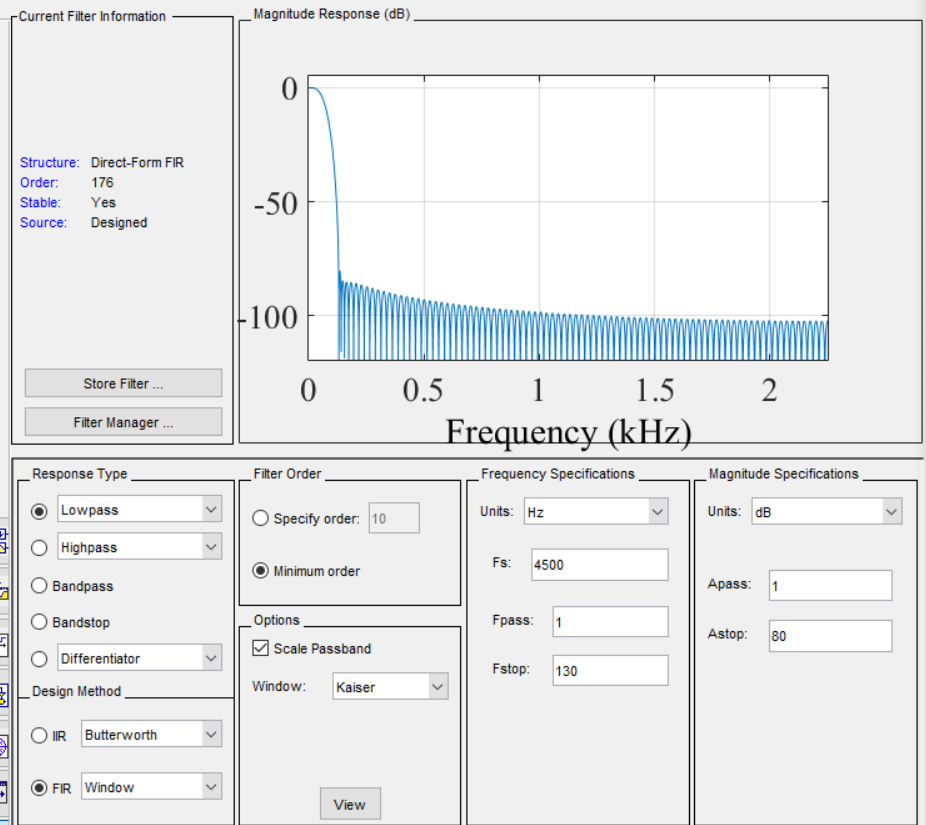
\includegraphics[width=150mm]{fdatool3}}
	\caption{Окно программы FDATool}
	\label{figCurves}
\end{figure}

\hspace{0,5cm}В результате был синтезирован фильтр $404$ порядка. 

\newpage
\begin{figure}[h]
	\begin{multicols}{1}
		\hfill
		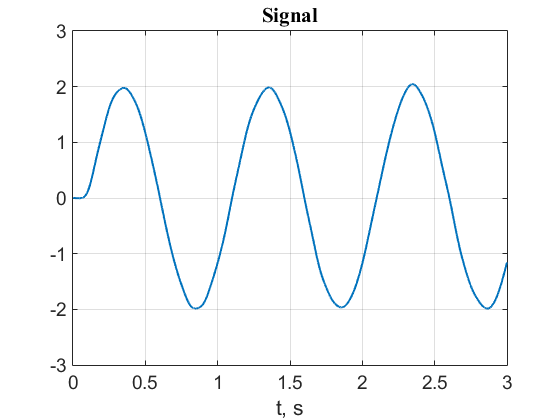
\includegraphics[width=90mm]{filtered3}
		\hfill
		\caption{Отфильтрованный сигнал}
		\label{figBottom}
		\hfill
		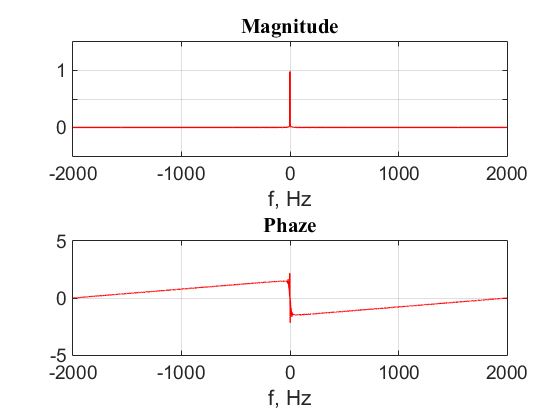
\includegraphics[width=100mm]{filtered_spec3}
		\hfill
		\caption{Спектры отфильтрованного сигнала}
		\label{figDown}
	\end{multicols}
\end{figure}

\subsection{Выводы}
\hspace{0,5cm}По итогам данной работы было получено, что при фильтрации сигнала частотой 2 Гц наилучший результат был получен при полосе проgускания равной 30 Гц. Это было проверено следующим образом: была взята полоса пропускания равная 300 Гц,  шум не был убран, затем полосу пропускания постепенно уменьшали, пока не был получен сигнал, практически с отсутствием шума. Однако, полученные параметры составляют фильтр 404 порядка, что не выгодно, при реализации данного фильтра. Такой фильтр нижних частот может пропускать низкочастотные шумы, поэтому для улучшения фильтрации может быть использован полосовой фильтр.

\end{document}